\documentclass[10pt]{llncs}
\usepackage{graphicx}
\usepackage{times}
\usepackage{amsmath}
\usepackage{amssymb}
\usepackage[hyphens]{url}
\usepackage{xspace}
\usepackage{microtype}
\usepackage{booktabs}
\usepackage{algorithm}
\usepackage{algpseudocode}
\usepackage{appendix}

% \usepackage[showframe]{geometry} % Solo para verificación, quitar en versión final
\usepackage{calc}
\usepackage{xcolor} % Para colores
\usepackage[colorlinks=true]{hyperref} % Enlaces clickeables
\hypersetup{
    linkcolor=blue,
    citecolor=blue,
    filecolor=blue,
    urlcolor=blue
}

% Personalización de referencias cruzadas
\usepackage{cleveref} % Paquete esencial

\crefname{figure}{Fig.}{Figs.} % Para figuras
\crefname{table}{Tab.}{Tabs.} % Para tablas
\crefname{equation}{Ec.}{Ecs.} % Para ecuaciones
\crefname{section}{Sec.}{Secs.} % Para secciones
% Configuración específica para tablas
\crefname{table}{Tab.}{Tabs.} % Singular y plural
\Crefname{table}{Tabla}{Tablas} % Para \Cref (inicio de oración)

% Configuración para LNCS (opcional)
\newcommand{\figref}[1]{\hyperref[#1]{Fig.~\ref*{#1}}}
\newcommand{\tabref}[1]{\hyperref[#1]{Tab.~\ref*{#1}}}
\newcommand{\secref}[1]{\hyperref[#1]{Sec.~\ref*{#1}}}
\newcommand{\AlgRef}[1]{\hyperref[#1]{Alg.~\ref{#1}}}


% Centrado completo del contenido (122mm x 193mm)
\setlength{\textwidth}{122mm}
\setlength{\textheight}{193mm}
\setlength{\oddsidemargin}{(\paperwidth - \textwidth)/2 - 1in}
\setlength{\evensidemargin}{(\paperwidth - \textwidth)/2 - 1in}
\setlength{\topmargin}{(\paperheight - \textheight - \headheight - \headsep - \footskip)/2 - 1in}

% Configuración adicional para cumplir requisitos
\setlength{\parindent}{0pt} % Sin sangría inicial
\frenchspacing % Espaciado adecuado después de puntos
\sloppy % Mejor manejo de división de palabras

% Abstract con márgenes de 1.0cm
\renewenvironment{abstract}{%
  \small
  \begin{list}{}{%
    \setlength{\leftmargin}{1cm}%
    \setlength{\rightmargin}{1cm}%
  }
  \item\relax\ignorespaces}
  {\end{list}\vspace{2\baselineskip}}

% Palabras clave
\newcommand{\keywords}[1]{\par\noindent\textbf{Keywords:} #1}

% Entorno para Remarks
% \newenvironment{remark}
%   {\par\noindent\textit{Remark.} \ignorespaces}
%   {\par}

% Configuración de figuras
\setlength{\abovecaptionskip}{8mm} % Espacio texto-figura
\setlength{\belowcaptionskip}{6mm} % Espacio figura-leyenda
\setlength{\textfloatsep}{10pt} % Espacio entre flotantes

\begin{document}

\title{GPTur}
\titlerunning{Título abreviado} % Sugerencia para running head

\author{Claudia Hernández Pérez \and Joel Aparicio Tamayo \and Kendry Javier Del Pino Barbosa}
\authorrunning{Autor1 et al.} % Apellidos para running head

\institute{
Facultad de Matemática y Computación, La Habana, Cuba
}

\maketitle

\begin{abstract} \textbf{Resumen.}
GPTur es un sistema diseñado con una arquitectura de Generación Aumentada por Recuperación (RAG) con agentes especializados para cada funcionalidad y una base de datos 
vectorial para la recuperación de la información. Posee, además, varios agentes encargados de tópicos específicos como gastronomía, 
vida nocturna, alojamiento y lugares históricos, que comparten datos en una pizarra central. Estos 
agentes están dirigidos por un guía y un planificador. El primero se encarga de responder consultas mientras el segundo utiliza algoritmos para planear 
itinerarios ajustados a presupuestos. Este agente resuelve un problema de satisfacción de restricciones utilizando la técnica de precocido simulado. También, el programa 
preprocesa la consulta para obtener ciertas entidades, palabras claves y sentimientos que puedan influir en los resultados esperados. Todo eso, permite conformar una respuesta acertada, 
acorde a las necesidades del usuario, validadas experimentalmente.
\par
\vspace{2\baselineskip}
\textbf{Palabras clave:} RAG, agente, problema de satisfacción de restricciones, precocido simulado
\end{abstract}

\section{Introducción}\label{sec:intro}
La industria turística enfrenta desafíos únicos en contextos con limitaciones en la infraestructura digital y 
actualización constante de servicios. Cuba, como destino turístico emblemático, requiere soluciones 
innovadoras que superen estas barreras mediante inteligencia artificial. \textit{GPTur}, 
un sistema de agentes inteligentes que funciona como guía turístico virtual, está diseñado específicamente 
para ser una alternativa viable en ese escenario.

La aplicación consiste en un chatbot capaz de responder consultas sobre destinos turísticos cubanos y sus peculiaridades, así como de generar itinerarios para \textit{tours} ajustándose a un presupuesto. 
El sistema está programado en \textit{Python}, aprovechando la comodidad del lenguaje y la diversidad de bibliotecas útiles que ofrece. La interfaz está diseñada con \textit{streamlit} (framework de \textit{Python} para \textit{frontend}), 
pues ofrece un estilo sencillo, moderno y fácil de programar para entornos web. El código fuente de la aplicación se puede encontrar en 
la plataforma GitHub: \href{https://github.com/ClaudiaHdezPerez/GPTur}{\color{blue}https://github.com/ClaudiaHdezPerez/GPTur}.

\section{Detalles de Implementación}\label{sec:implementacion}

En esta sección, se abordarán los distintos temas asociados a la implementación de la solución propuesta, que incluyen la arquitecura RAG y multiagente, funcionamiento del \textit{crawler} automatizado y recopilación del corpus, base de datos vactorial y representación semántica del 
conocimiento mediante \textit{embeddings}, procesamiento de lenguaje natural, algoritmos basados en metaheurísticas, entre otros. 

\vspace{\baselineskip}

\subsection{Arquitectura RAG (\textit{Generación Aumentada por Recuperación})}\label{sec:rag}

Un sistema de Generación Aumentada por Recuperación combina generación de texto con recuperación de información para mejorar la calidad, precisión y actualidad de las respuestas obtenidas de los modelos de lenguaje. 
Está compuesto por una entrada, un recuperador, un generador y una salida. La implementación propuesta es bastante sencilla, ajustada a la definición:
\begin{enumerate}
    \item Entrada: constituida por la consulta del usuario en lenguaje natural.
    \item Recuperador: agente que recibe la consulta y le pide a la base de datos vectorial que recupere la información relacionada.
    \item Generador: agente que utiliza la consulta y la información recuperada para decidir si la respuesta debe ser generada por el guía o el planificador. Para tomar esa decisión le pide a un modelo de lenguaje que detecte la intención del usuario.
    \item Salida: respuesta generada por el agente inteligente encargado de elaborarla.
\end{enumerate}

\vspace{\baselineskip}
\subsection{Arquitectura multiagente}

Un sistema multiagente está constituido por un conjunto de agentes, cada uno con determinadas capacidades y recursos para la solución de problemas inherentemente distribuidos. Los agentes interactúan entre ellos, determinan y coordinan tareas a realizar según sus capacidades y recursos.

GPTur cuenta con dos agentes fundamentales: el guía y el planificador. Existen, además, 
otros especializados en distintos tópicos: gastronomía, vida nocturna, alojamiento y lugares históricos. Todos ellos 

\vspace{\baselineskip}
\subsection{Crawler Automatizado en Dos Fases. Recopilación del \textit{Corpus}}

Se conoce como \textit{crawler} a un software que realiza un proceso automatizado de navegar por la Web de manera sistemática para indexar y recopilar
información de diferentes sitios web. El sistema implementa un \textit{crawler} en dos fases:
\begin{itemize}
  \item  \textit{Fase inicial:} Recopila, almacena y organiza datos en un repositorio vectorial,
 garantizando una gestión eficiente de los vectores de información.
  \item \textit{Fase dinámica:} Utiliza automáticamente información externa cuando el sistema
 detecte respuestas incompletas o desactualizadas.
\end{itemize}

\subsubsection{Fase Inicial:} En esta fase el \textit{crawler} se configura con los parámetros necesarios, como las URLs objetivo (disponibles en \textit{src /data /sources.json}), 
criterios de búsqueda y profundidad de rastreo. Utiliza técnicas de \textit{scraping} (extracción de la web) para navegar por sitios web turísticos, identificando y extrayendo 
información relevante como descripciones de lugares, eventos, alojamientos y actividades. Los datos extraídos son normalizados y almacenados en un formato \textit{.json}, facilitando su posterior análisis y procesamiento.

\subsubsection{Fase Dinámica:} Esta fase actúa cuando el programa detecta que la información con que cuenta no es suficiente para responder concretamente la consulta del usuario. Esta detección es realizada por un modelo de 
lenguaje al cual se le envía un \textit{prompt} con la consulta y los documentos relevantes encontrados, esperando una respuesta de \textit{OK} o \textit{Actualizar}. En caso de la segunda, en un nuevo \textit{prompt} se le pide 
\textit{urls} que permitan enriquecer el corpus y responder la consulta. El \textit{crawler} accede a ellas y se toma dicha información para continuar el proceso del programa. A su vez dicha información es añadida a la base de datos 
vectorial.

\subsubsection{Recopilación y Construcción del Corpus:} Este proceso consta de cuatro tareas principales:

\begin{itemize}
    \item \textit{Selección de Fuentes:} Se identificaron y seleccionaron fuentes web relevantes para el turismo, como portales oficiales, blogs y sitios de reseñas.
    \item \textit{Rastreo y Descarga:} El \textit{crawler} recorre las páginas seleccionadas, descargando el contenido textual y metadatos asociados.
    \item \textit{Filtrado y Normalización:} Se aplican filtros para eliminar información irrelevante o duplicada, y se normalizan los datos para mantener la coherencia en el corpus.
    \item \textit{Almacenamiento:} El corpus final se almacena en formato \textit{.json} (disponible en \textit{src /data /processed /normalized\_data.json}).
\end{itemize}

Este proceso automatizado permite mantener un corpus representativo del dominio turístico, esencial para el tema que aborda el sistema.

\vspace{\baselineskip}
\subsection{Base de Datos Vectorial y Modelo de Representación del Conocimiento}

El sistema utiliza \textit{ChromaDB} como base de datos vectorial. \textit{ChromaDB} es una solución 
especializada para el almacenamiento y consulta de vectores de alta dimensión, optimizada para tareas de inteligencia artificial y procesamiento de lenguaje natural.

\begin{itemize}
    \item \textit{Integración con el Sistema:} La integración se realiza a través del módulo \newline\textit{src /vector\_db /chroma\_storage.py}, que proporciona funciones para insertar, actualizar y consultar vectores en la base de datos.
    \item \textit{Almacenamiento Eficiente:} \textit{ChromaDB} permite almacenar grandes volúmenes de \textit{embeddings} generados a partir del corpus, manteniendo tiempos de respuesta bajos incluso en consultas complejas.
    \item \textit{Búsqueda por Similitud:} Utilizando algoritmos de búsqueda aproximada de vecinos más cercanos (ANN), \textit{ChromaDB} facilita la recuperación de fragmentos de información relevantes a partir de consultas vectorizadas, mejorando la precisión y relevancia de las respuestas del sistema.
    \item \textit{Escalabilidad y Actualización:} \textit{ChromaDB} soporta la actualización dinámica de la base de datos, permitiendo añadir o eliminar vectores conforme el corpus evoluciona, sin afectar el rendimiento general.
    \item \textit{Persistencia y Seguridad:} Los datos almacenados en \textit{ChromaDB} pueden persistirse en disco, asegurando la integridad y disponibilidad de la información incluso ante reinicios del sistema.
\end{itemize}

El uso de \textit{ChromaDB} proporciona una infraestructura robusta y escalable para la gestión del conocimiento en forma vectorial, facilitando la integración de capacidades avanzadas de recuperación semántica y razonamiento en el sistema.

\subsubsection{Modelo de Representación del Conocimiento:}

El sistema emplea un modelo de representación del conocimiento basado en \textit{embeddings} semánticos, lo que permite capturar relaciones y similitudes entre conceptos turísticos. Las principales características son:

\begin{itemize}
    \item \textit{Representación Distribuida:} Cada entidad o fragmento de información se representa como un vector en un espacio de alta dimensión, facilitando la comparación y agrupación de conceptos similares.
    \item \textit{Recuperación Semántica:} Las consultas del usuario se transforman en vectores y se comparan con los almacenados en la base de datos, recuperando la información más relevante según la similitud semántica. Todo 
    eso gracias al método \textit{similarity\_search} de \textit{Chroma}.
\end{itemize}

Este enfoque permite una gestión eficiente y flexible del conocimiento, adaptándose a la naturaleza dinámica y heterogénea de la información turística.

\vspace{\baselineskip}
\subsection{Procesamiento de Lenguaje Natural (NLP)}

El sistema GPTur incorpora un módulo de procesamiento de lenguaje natural (NLP) para analizar y comprender las consultas de los usuarios, así como para procesar y organizar la información turística recopilada. Las principales tareas de 
NLP implementadas son:

\begin{itemize}
    \item \textit{Preprocesamiento de texto:} Se realiza limpieza, normalización y lematización de las consultas y documentos, eliminando palabras vacías y signos de puntuación, utilizando el modelo \textit{es\_core\_news\_md} de \textit{spacy}.
    \item \textit{Extracción de entidades:} Se identifican entidades nombradas relevantes (como ciudades, atracciones y organizaciones) en las consultas y documentos, facilitando la recuperación precisa de información.
    \item \textit{Análisis de sentimiento:} Se implementa un análisis de sentimiento simple para detectar la polaridad de las consultas, lo que puede influir en la generación de respuestas más adecuadas.
    \item \textit{Extracción de palabras clave:} Se extraen los términos más relevantes de cada consulta o documento, mejorando la indexación y recuperación.
    \item \textit{Fragmentación de texto:} Los textos largos se dividen en fragmentos coherentes para optimizar el procesamiento y la generación de embeddings.
\end{itemize}

Estas tareas permiten que el sistema interprete correctamente las necesidades del usuario y recupere la información más relevante, integrando el procesamiento de lenguaje natural en la lógica central de los agentes inteligentes.

\vspace{\baselineskip}

\subsection{Metaheurística y Problema de Satisfacción de Restricciones}

%...

En el desarrollo de sistemas de planificación de viajes inteligentes, surge el problema de optimizar itinerarios turísticos considerando múltiples restricciones y objetivos.

El sistema debe generar un itinerario diario considerando:
\begin{itemize}
    \item \textit{Actividades:} Desayuno, almuerzo, cena, actividad nocturna y alojamiento.
    \item \textit{Restricciones:} Presupuesto diario máximo.
    \item \textit{Objetivo:}Maximizar la valoración total de los lugares seleccionados.
\end{itemize}

Matemáticamente, el problema se formula como:

\[
\max \sum_{d=1}^{D} \sum_{a \in A} r_{d,a}
\]
\[
\text{sujeto a: }
\sum_{a \in A} c_{d,a} \leq B_d \quad \forall d \in \{1,\dots,D\}
\]

Donde:
\begin{itemize}
    \item $D$: Número de días del viaje
    \item $A = \{\text{desayuno}, \text{almuerzo}, \text{cena}, \text{noche}, \text{alojamiento}\}$
    \item $r_{d,a}$: Valoración del lugar asignado al día $d$ para actividad $a$
    \item $c_{d,a}$: Costo del lugar asignado al día $d$ para actividad $a$
    \item $B_d$: Presupuesto máximo para el día $d$
\end{itemize}

\subsubsection{Algoritmo de Recocido Simulado:}
El recocido simulado es una metaheurística inspirada en el proceso térmico de recocido en metalurgia. Para el problema en cuestión pudiese surgir la 
interrogante de por qué utilizar metaheurística para resolver un problema de optimización lineal. La respuesta es simplemente porque los costos asociados a cada 
lugar están representados por un proceso estocástico, que representa situaciones reales, como ofertas, descuentos, diferencia de precios según la época del año, los 
fines de semana, en fin, un conjunto de situaciones que evitan que los precios sean estáticos. A continuación se describe la implementación del algoritmo.

\paragraph{Representación de la Solución:}
Cada solución se representa como una matriz donde las filas corresponden a días y las columnas a tipos de actividad:

\begin{center}
\begin{tabular}{c|c|c|c|c|c}
Día & Desayuno & Almuerzo & Cena & Noche & Alojamiento \\
\midrule
1 & $L_{11}$ & $L_{12}$ & $L_{13}$ & $L_{14}$ & $L_{15}$ \\
2 & $L_{21}$ & $L_{22}$ & $L_{23}$ & $L_{24}$ & $L_{25}$ \\
$\vdots$ & $\vdots$ & $\vdots$ & $\vdots$ & $\vdots$ & $\vdots$ \\
\end{tabular}
\end{center}

Donde $L_{ij}$ es un lugar seleccionado del conjunto correspondiente a la categoría.

\paragraph{Función de Evaluación:}
La calidad de una solución se calcula como la suma de las valoraciones de todos los lugares seleccionados:

\[
f(S) = \sum_{d=1}^{D} \sum_{a \in A} \text{rating}(L_{d,a})
\]

\paragraph{Generación de Vecinos:}
El operador de vecindad modifica aleatoriamente una actividad en un día. Ver \AlgRef{alg:nb_gen}.

\paragraph{Esquema de Enfriamiento:}
Se utiliza un enfriamiento geométrico:

\[
T_{k+1} = \alpha \cdot T_k \quad \text{con} \quad \alpha = 0.99
\]

Parámetros iniciales:
\begin{itemize}
    \item Temperatura inicial ($T_0$): 100.0
    \item Temperatura mínima ($T_{\min}$): 0.1
    \item Iteraciones por temperatura: 1000
\end{itemize}

\paragraph{Manejo de Restricciones:}
Las soluciones se validan verificando que el costo diario total no exceda el presupuesto. Ver \AlgRef{alg:sol_valid}.

\paragraph{Implementación:}
La implementación completa se puede apreciar en el \AlgRef{alg:recocido_viajes}.


\vspace{\baselineskip}
\section{Validación y Experimentación}


\vspace{\baselineskip}



Esta sección fue un elemento esencial en la etapa de desarrollo y, en muchos casos, influyó en la toma de decisiones. Se realizaron varios experimentos, que incluyen valoraciones de la respuesta del sistema y evaluación de los algoritmos de metaheurísticas.

\vspace{\baselineskip}
\subsection{Respuesta del Sistema}

Durante las distintas etapas de desarrollo, fue importante evaluar el comportamiento de la aplicación. Para estos experimentos se utilizó un modelo de lenguaje para generar 30 preguntas relacionadas con el corpus y obtener las respuestas de GPTur automáticamente. Luego, 
se creó una cosulta para un modelo de lenguaje pidiendo una evaluación entre 0 y 5 puntos de la respuesta del sistema en cuanto a:
\begin{itemize}
    \item  Precisión de la información
    \item Coherencia y relevancia
    \item Cobertura del tema
    \item Calidad de las recomendaciones
    \item Ajuste a la pregunta realizada
\end{itemize}

Después de obtener los resultados de la muestra original, se llegó a la conclusión de que se debían analizar muchas más muestras, es decir, ejecutar la experimentación varias veces, pero la capacidad de cómputo y tiempo necesarios para generar 30 preguntas y evaluar las respuestas un número \textit{n} de veces, con \textit{n} relativamente 
grande, hacían inviable esa solución. Por tanto, se recurrió a una alternativa no menos eficaz: simular la evaluación de nuevas muestras. Es entonces cuando se decidió aplicar la técnica conocida como \textit{bootstrapping}.

\subsubsection{Procedimiento de Bootstrapping y Número de Iteraciones:}

En el procedimiento de bootstrapping se generan, con reemplazamiento, $B$ muestras de tamaño $n$ a partir de la muestra original, calculándose de cada una el estimador $\bar{X}^*$.
El error estándar asociado a la distribución de estos estimadores se expresa como:
\begin{equation}
\text{SE}_B = \frac{\sigma}{\sqrt{B}}.
\end{equation}
Para los experimentos realizados utilizando esta técnica, inicialmente se había planteado un umbral del 5\% de $\sigma$, para que $\text{SE}_B$ fuese insignificante comparado con la variabilidad natural de los datos, lo que implicaba:
\begin{equation}
\text{SE}_B \leq 0.05\,\sigma.
\end{equation}
Despejando en la inecuación se obtiene


\[
\frac{\sigma}{\sqrt{B}} \leq 0.05\,\sigma \quad \Longrightarrow \quad \sqrt{B} \geq 20 \quad \Longrightarrow \quad B \geq 400.
\]


Entonces, para mantener el error estándar por debajo del umbral propuesto, en cada experimento se debió realizar al menos 400 simulaciones. Sin embargo, se tomó la decisión de 
hacer 1000 en total, para hacer más robusto el experimento y dismnuir aún más el error estándar:


\[
\frac{1}{\sqrt{1000}} \approx 0.0316,
\]


lo que implica que $\text{SE}_B\approx 0.0316\,\sigma$, cumpliéndose de forma estricta la condición.


\subsubsection{Sistema con Agentes Guía y Planificador Solamente:}

La Tabla \tabref{tab:boot_results_1} resume las métricas clave obtenidas:

\begin{table}[h]
\centering
\caption{Resultados del análisis de bootstrapping (IC 95\%)}
\label{tab:boot_results_1}
\begin{tabular}{lccc}
\hline
\textbf{Métrica} & \textbf{Original} & \textbf{Bootstrapped}  \\
\hline 
Puntuación Media& 3.7 & 3.6982...  \\
Desviación Estándar & 0.4582... & 0.0839...  \\
\hline
\end{tabular}
\end{table}

\begin{remark}
Se obtuvo un intervalo de confianza de $[3.5333..., 3.8666...]$, lo que indica unos resultados aceptables. 
La Figura {\figref{fig:boot_dist_1}} muestra la distribución bootstrap de la puntuación media y la figura
{\figref{fig:eval_1}} muestra un mapa de calor con las puntuaciones otorgadas a las respuestas del sistema a las 
30 preguntas iniciales.
\end{remark}

\subsubsection{Sistema con Agentes Especializados:}

La Tabla \tabref{tab:boot_results_2} resume las métricas clave obtenidas:

\begin{table}[h]
\centering
\caption{Resultados del análisis de bootstrapping (IC 95\%)}
\label{tab:boot_results_2}
\begin{tabular}{lccc}
\hline
\textbf{Métrica} & \textbf{Original} & \textbf{Bootstrapped}  \\
\hline 
Puntuación Media& 4.1333... & 4.1358...  \\
Desviación Estándar & 0.6182... & 0.1166...  \\
\hline
\end{tabular}
\end{table}

\begin{remark}
Se obtuvo un intervalo de confianza de $[3.90,4.3666...]$, lo que indica unos resultados bastante buenos. 
La Figura {\figref{fig:boot_dist_2}} muestra la distribución bootstrap de la puntuación media y la figura 
{\figref{fig:eval_2}} muestra un mapa de calor con las puntuaciones otorgadas a las respuestas del sistema a las 
30 preguntas iniciales.
\end{remark}

En resumen, se puede observar que al añadir agentes especializados al sistema, mejoró la respuesta del modelo, lo cual demostró 
que la decisión tomada estuvo acertada.

\vspace{\baselineskip}
\section{Conclusiones}


GPTur constituye un sistema robusto, ideal como proyecto de carácter educativo para estudiantes de Ciencias de la Computación, pues fomentó 
la investigación, recolección y almacenamiento de datos, ingeniería de software, trabajo en equipo y la experimentación, que son las habilidades que la carrera busca impregnar en cada 
estudiante. No obstante, su interfaz amigable, sus respuestas actualizadas y personalizadas, así como su arquitectura escalable, abren las puertas a futuras aplicaciones que mejoren la experiencia de los turistas en la Isla.

La eficacia del sistema no solo se basa en resultados subjetivos, sino que está respaldada por un conjunto de pruebas y experimentos que han demostrado cómo ha ido evolucionando GPTur, incrementando la precisión de sus respuestas en cada fase 
de desarrollo, lo que justifica las decisiones tomadas para la implementación propuesta.

La aplicación es una muestra del esfuerzo de todo un semestre y de los conocimientos adquiridos en los temas de \textit{Simulación}, \textit{Inteligencia Artificial} y \textit{Sistemas de Recuperación de Información}, pues en tiempo record se logró 
implementar un RAG, una arquitectura multiagente, metaheurística, entre otros muchos aspectos, que debieron ser quirúrjicamente enlazados para el funcionamiento completo del programa.

Por supuesto, como todo sistema, tiene limitaciones que no pudieron resolverse en el tiempo especificado:
\begin{itemize}
    \item No considerar las distancias entre los sitios a la hora de planear viajes utilizando la metaheurística.
    \item No considerar el transporte como elemento fundamental en los \textit{tours}.
    \item No utilizar ontologías para realizar inferencias sobre los sentimientos e intenciones del usuario.
\end{itemize}

No obstante, se proponen algunas soluciones para lograrlas:
\begin{itemize}
    \item Integrar el sistema a una API con datos sobre la ubicación de sitios turísticos y permita calcular distancias.
    \item Añadir nuevos agentes especializados para manejar otros problemas, como por ejemplo el del transporte.
    \item Integrar una ontología o un sistema basado en reglas para captar mejor las intenciones del usuario.
\end{itemize}

Por todo lo expuesto y más, GPTur ha llegado a ser una experiencia magnífica para cada uno de sus desarrolladores.

% ===== INICIO DE APÉNDICES =====
\newpage
\section{Apéndices}
A continuación se muestran los apéndices del informe.
\appendix

% --- Apéndice A ---
\section{Estudios Estadísticos}

\begin{figure}
\centering
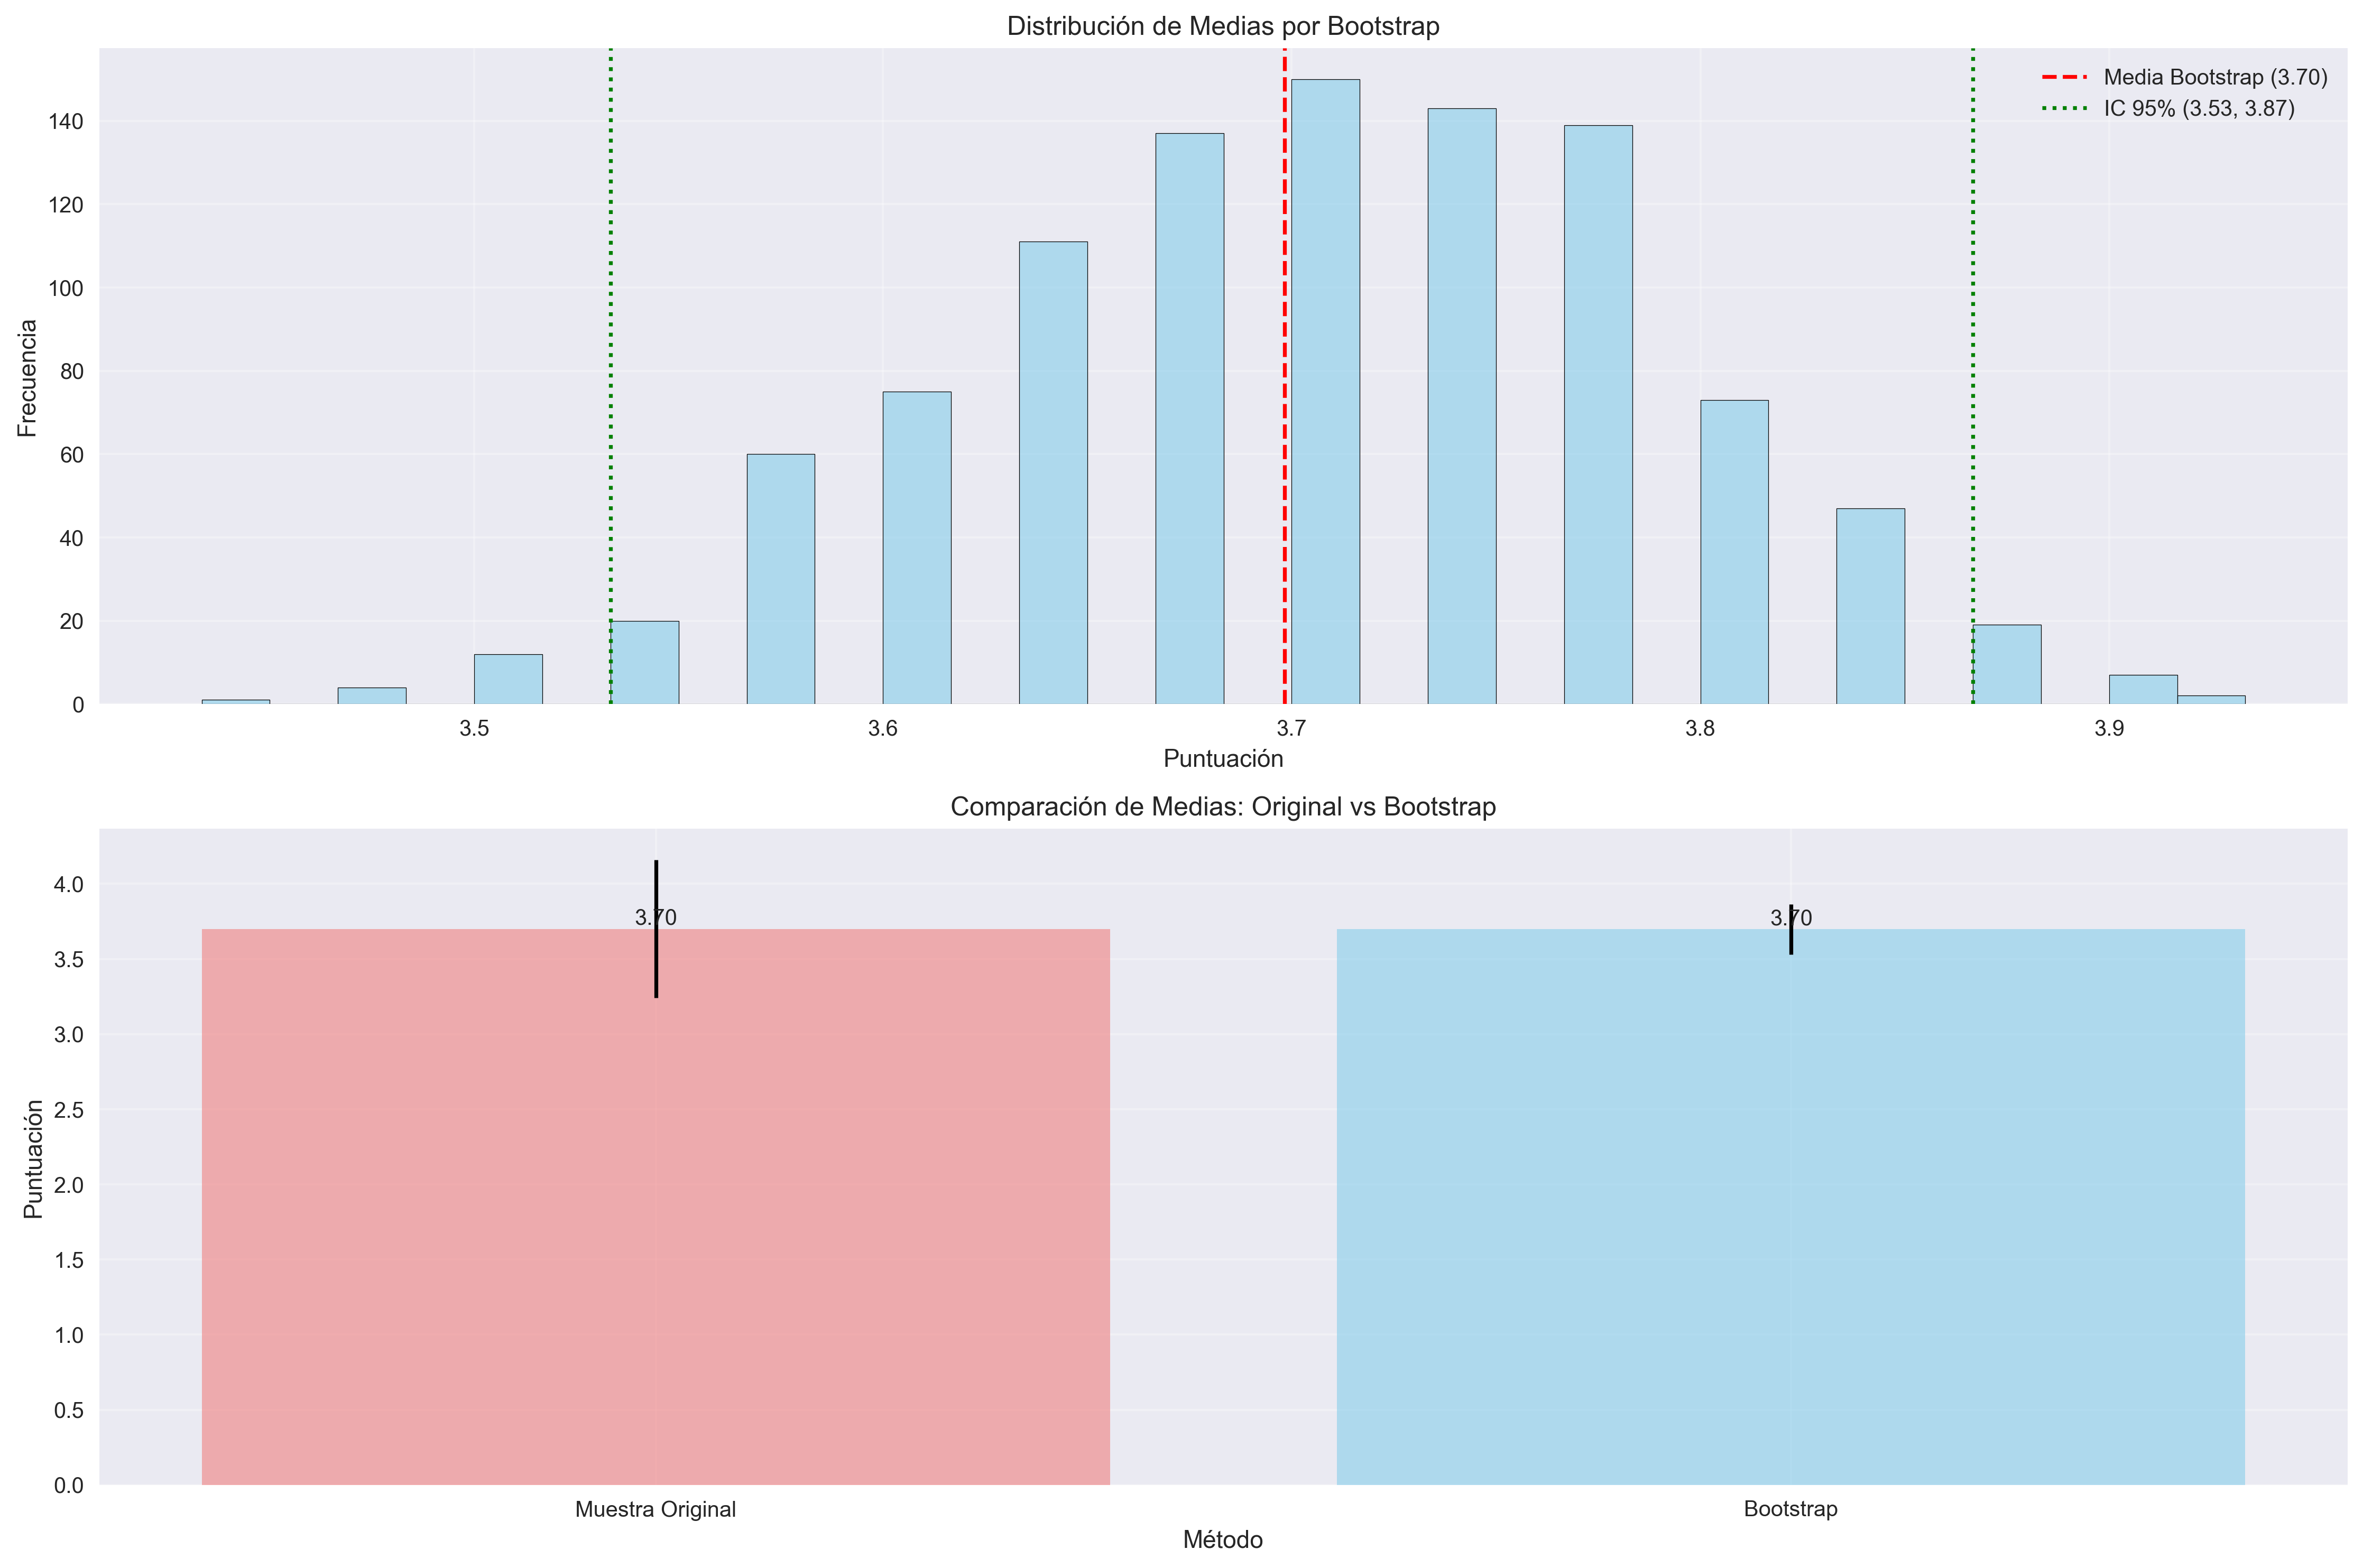
\includegraphics[width=1\textwidth]{../src/experiments/one_only_agent/bootstrap_distribution_20250617-171514.png}
\caption{Distribución bootstrap de la puntuación media ($N=1000$). La línea discontinua roja indica la media bootstrap (3.70)}
\label{fig:boot_dist_1}
\end{figure}

\begin{figure}
\centering
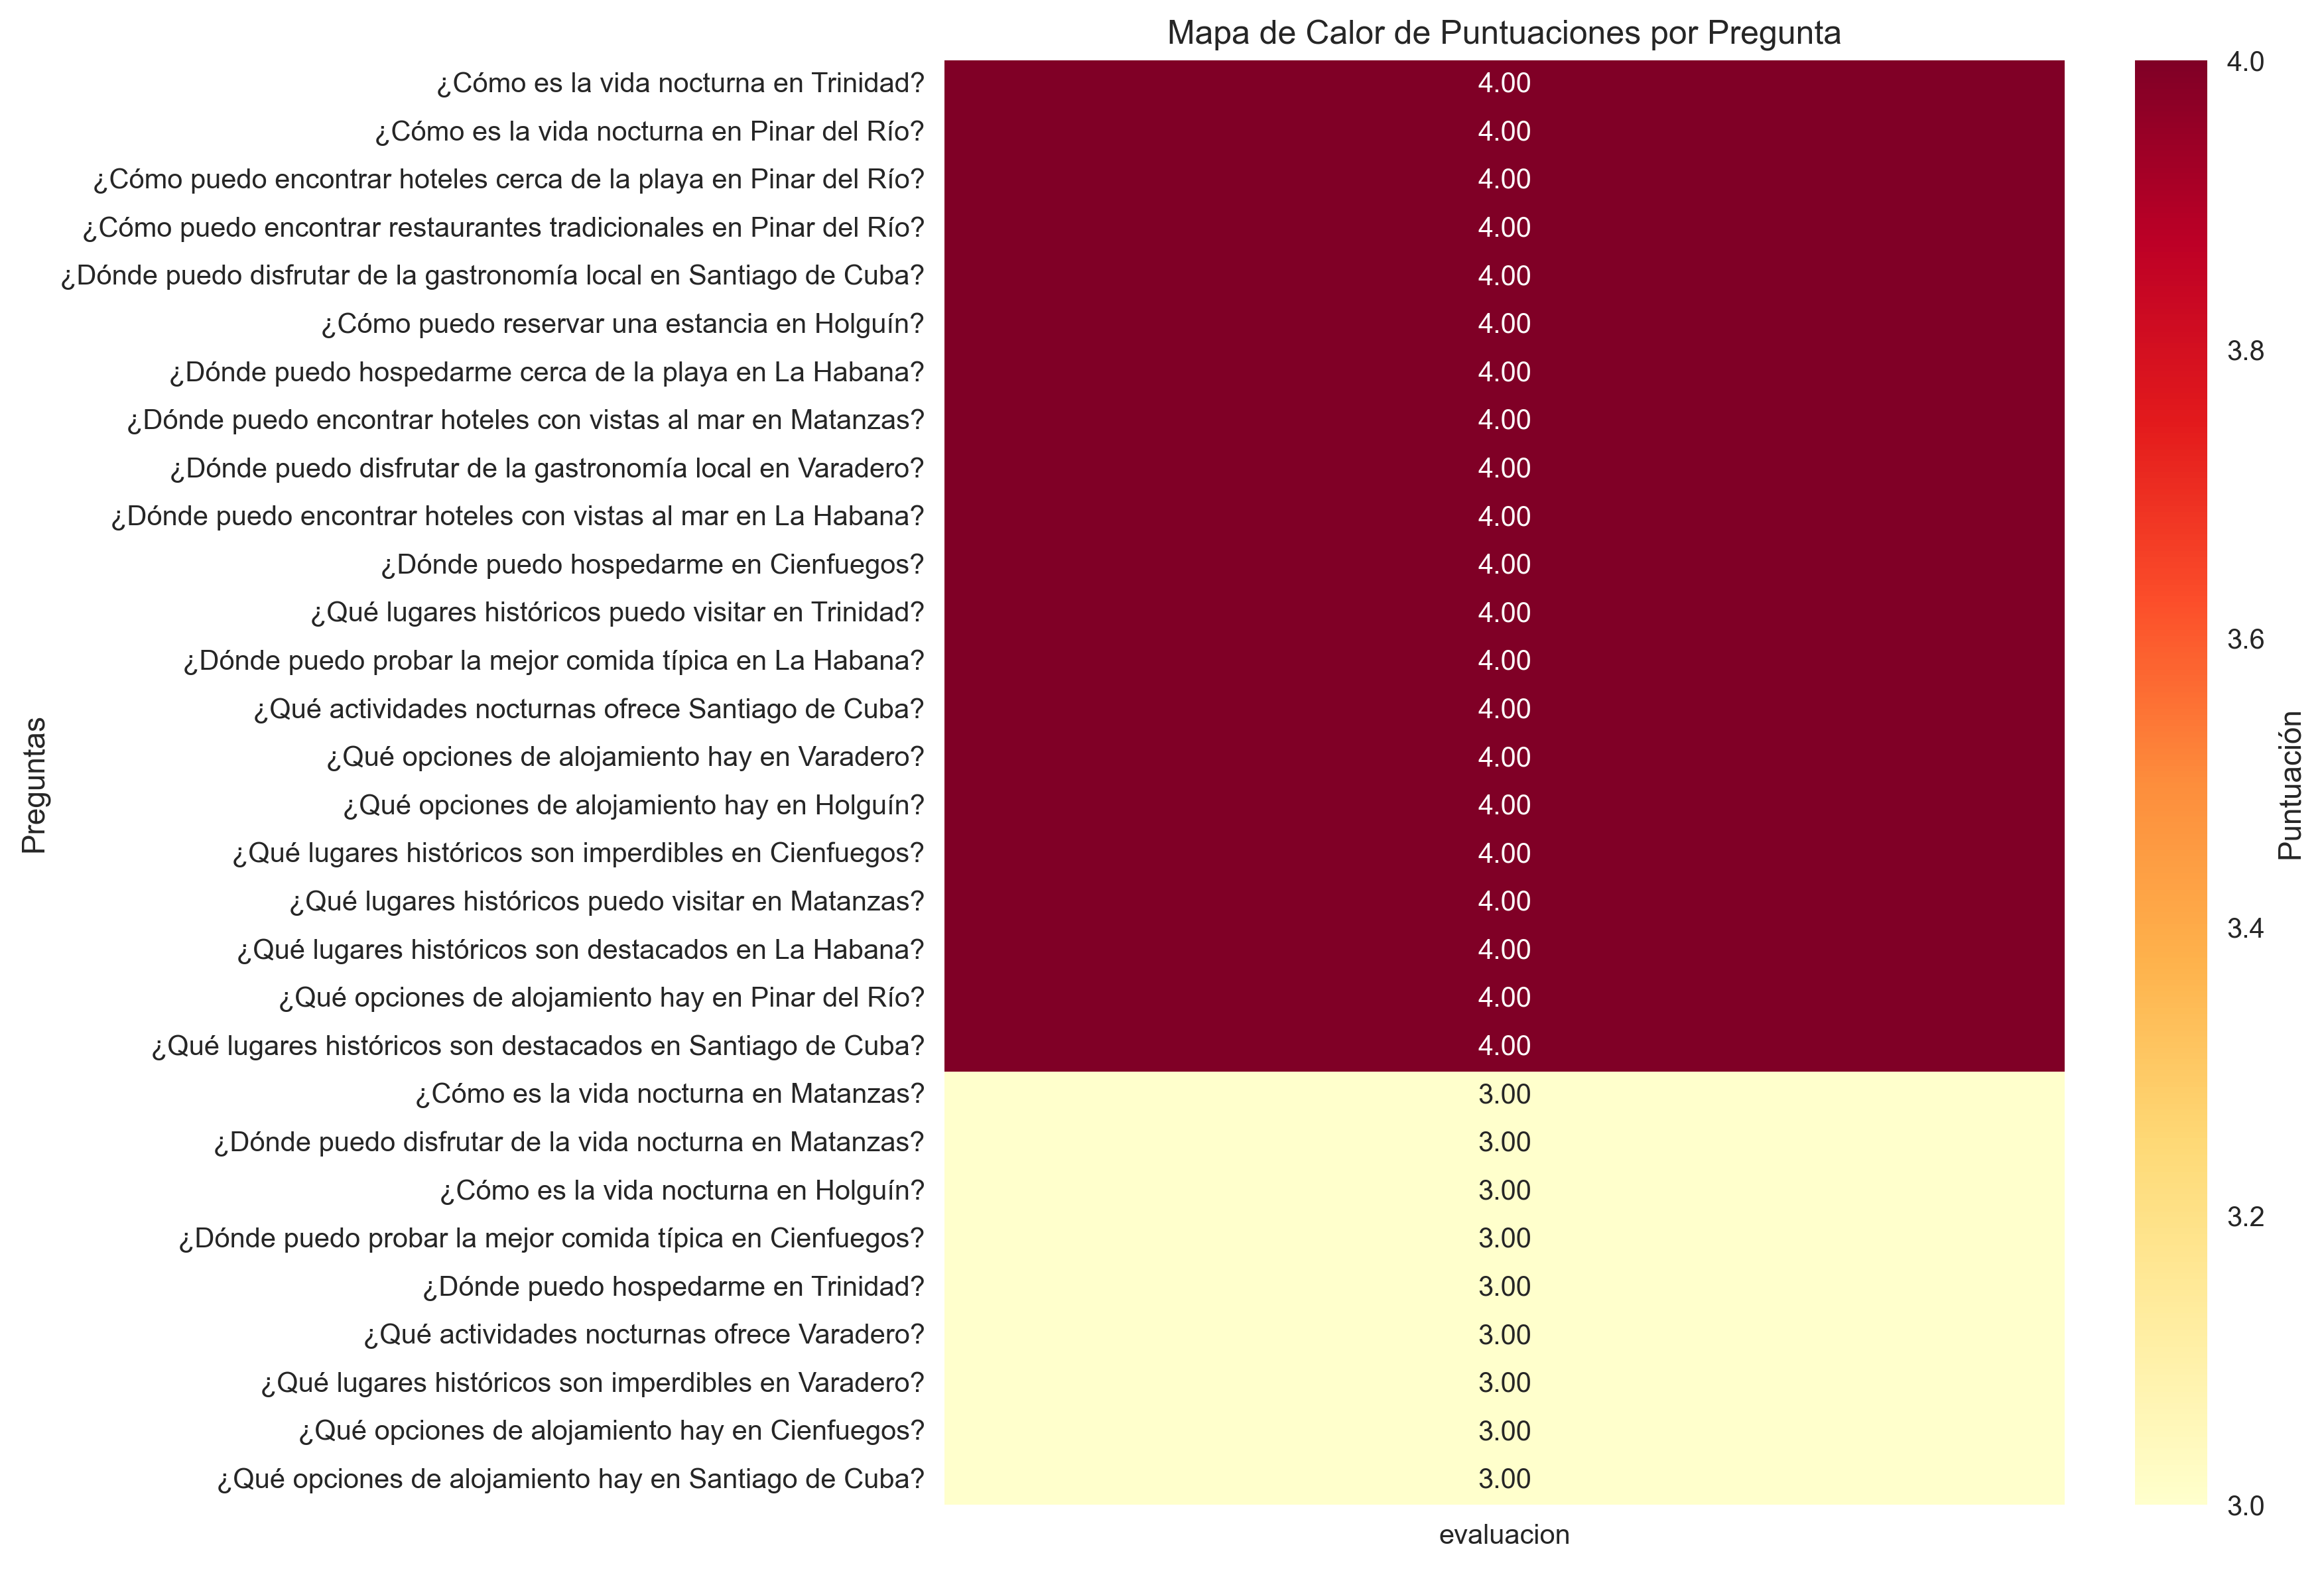
\includegraphics[width=1\textwidth]{../src/experiments/one_only_agent/quality_heatmap_20250617-171514.png}
\caption{Evaluaciones obtenidas para la respuesta a cada pregunta en la muestra inicial (tamaño 30)}
\label{fig:eval_1}
\end{figure}

\begin{figure}
\centering
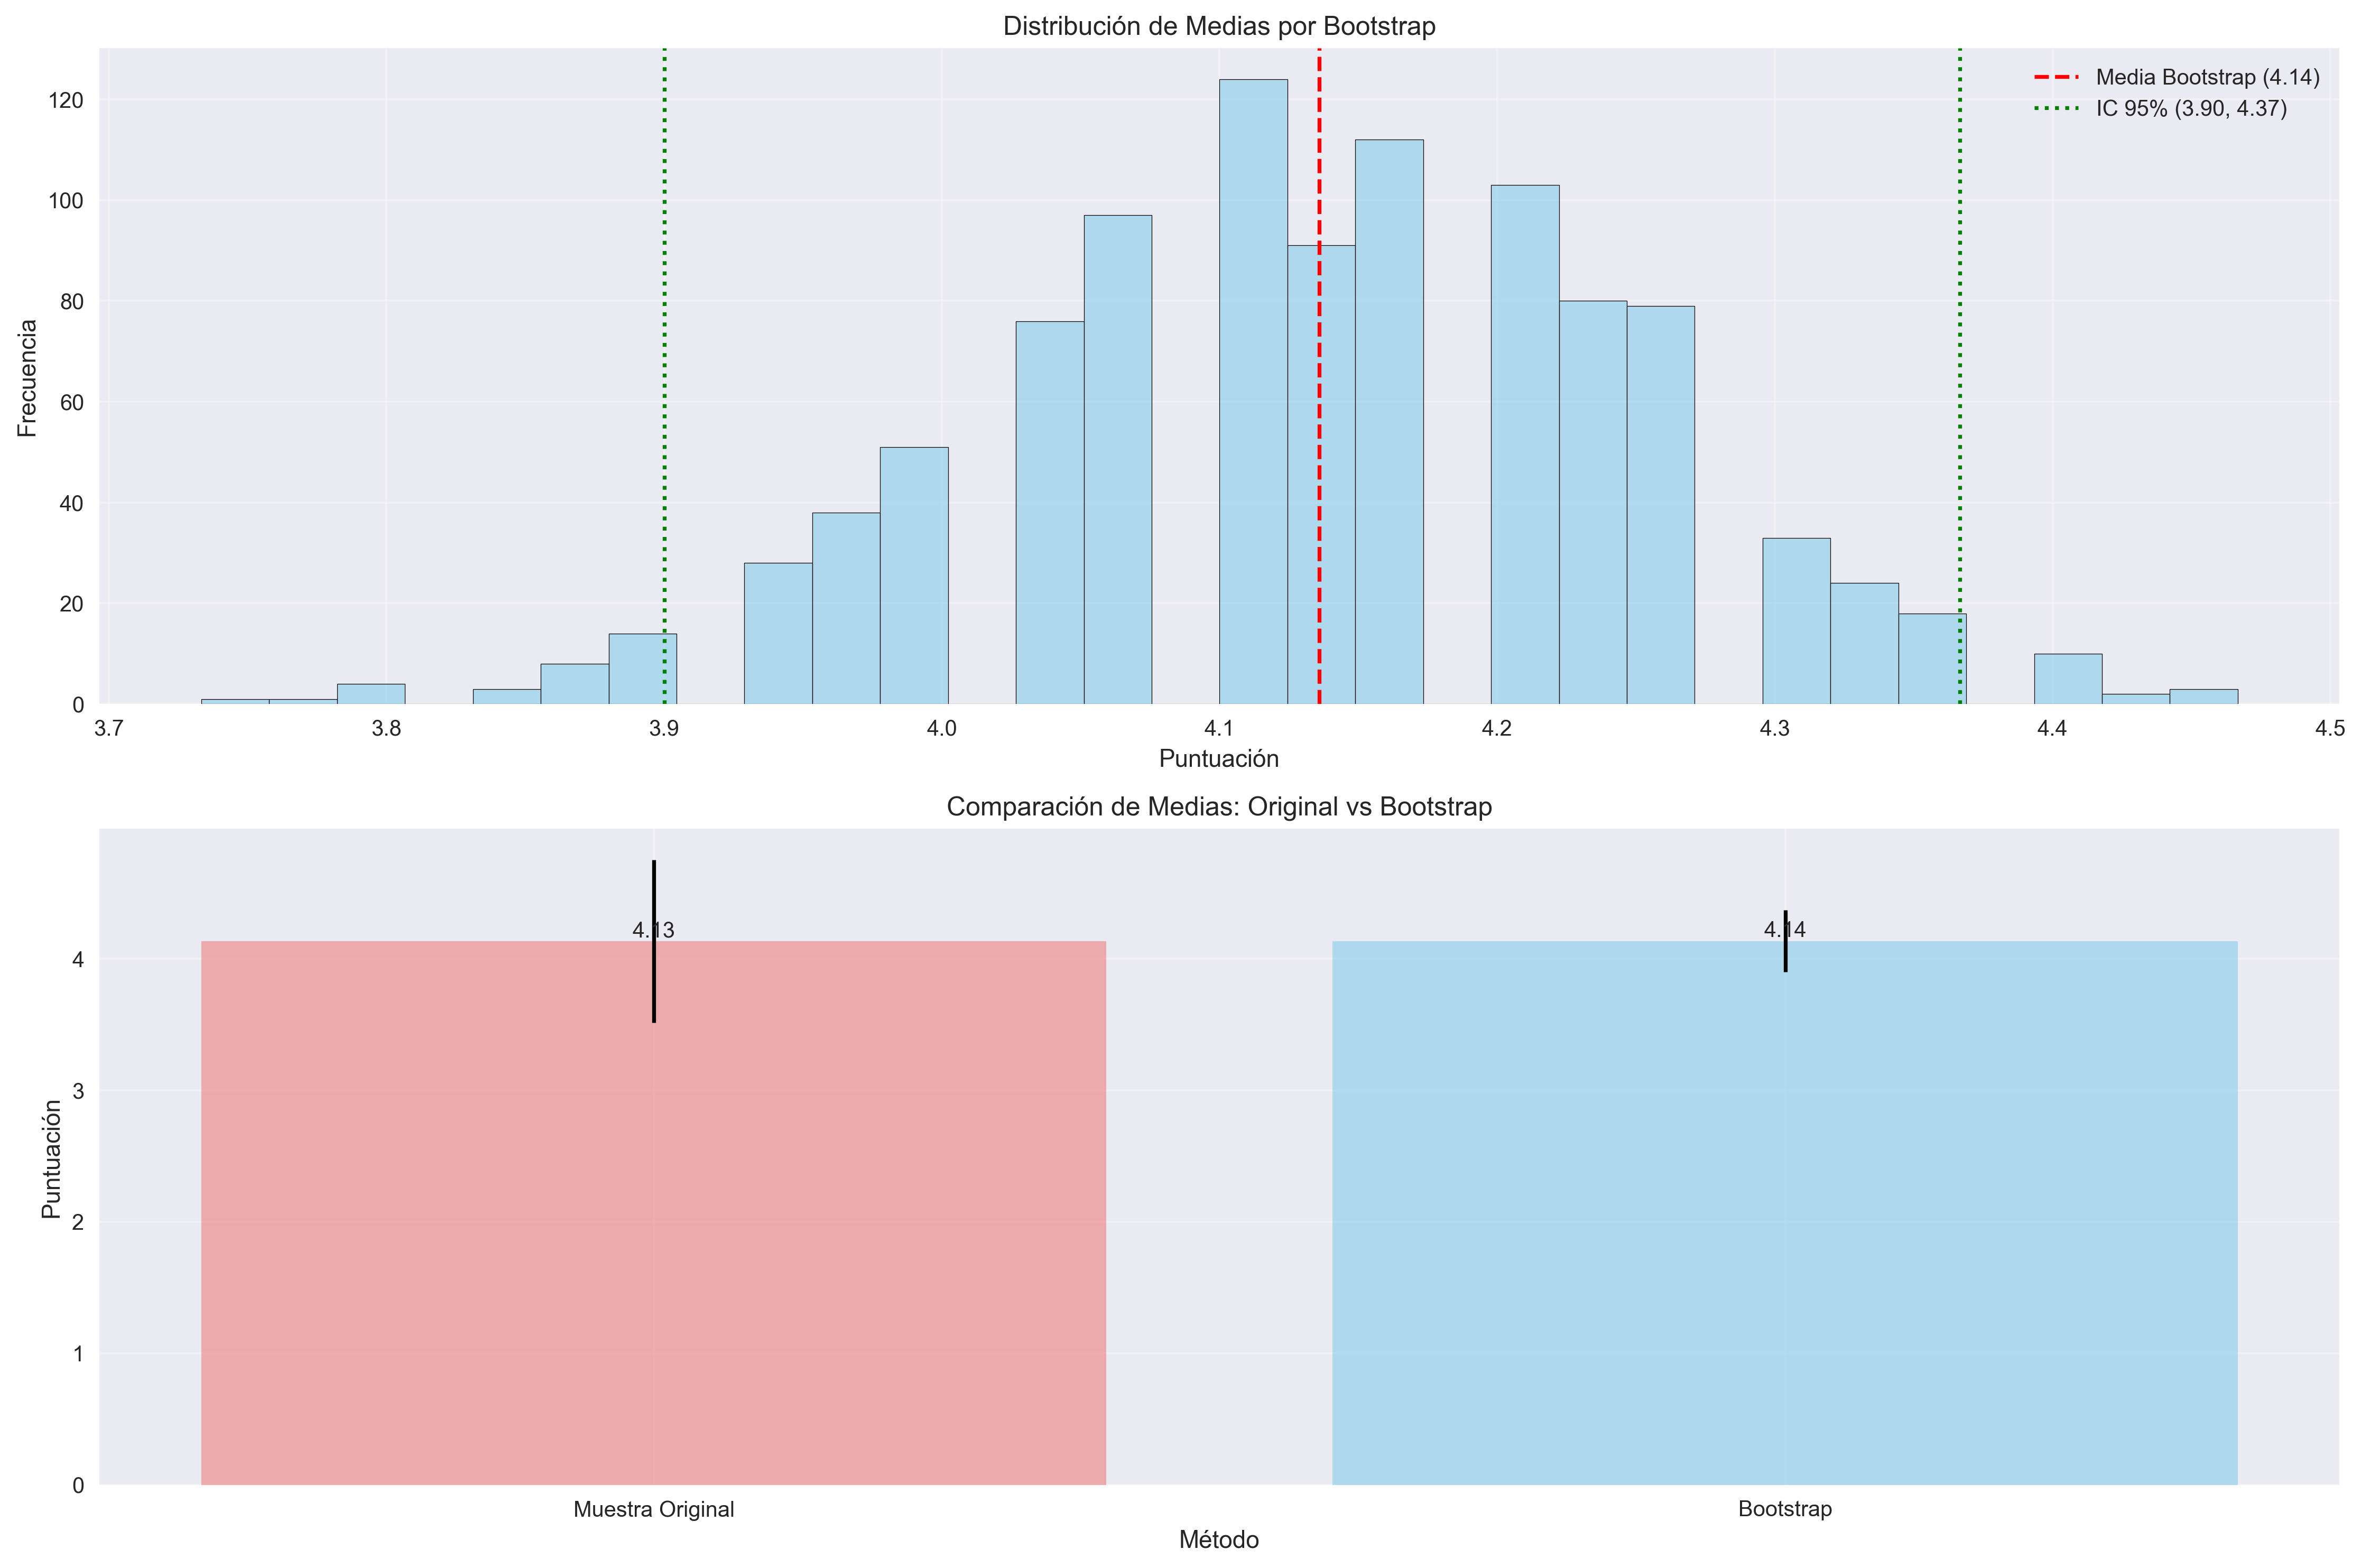
\includegraphics[width=1\textwidth]{../src/experiments/specialized_agents/bootstrap_distribution_20250617-171856.png}
\caption{Distribución bootstrap de la puntuación media ($N=1000$). La línea discontinua roja indica la media bootstrap (4.14)}
\label{fig:boot_dist_2}
\end{figure}

\begin{figure}
\centering
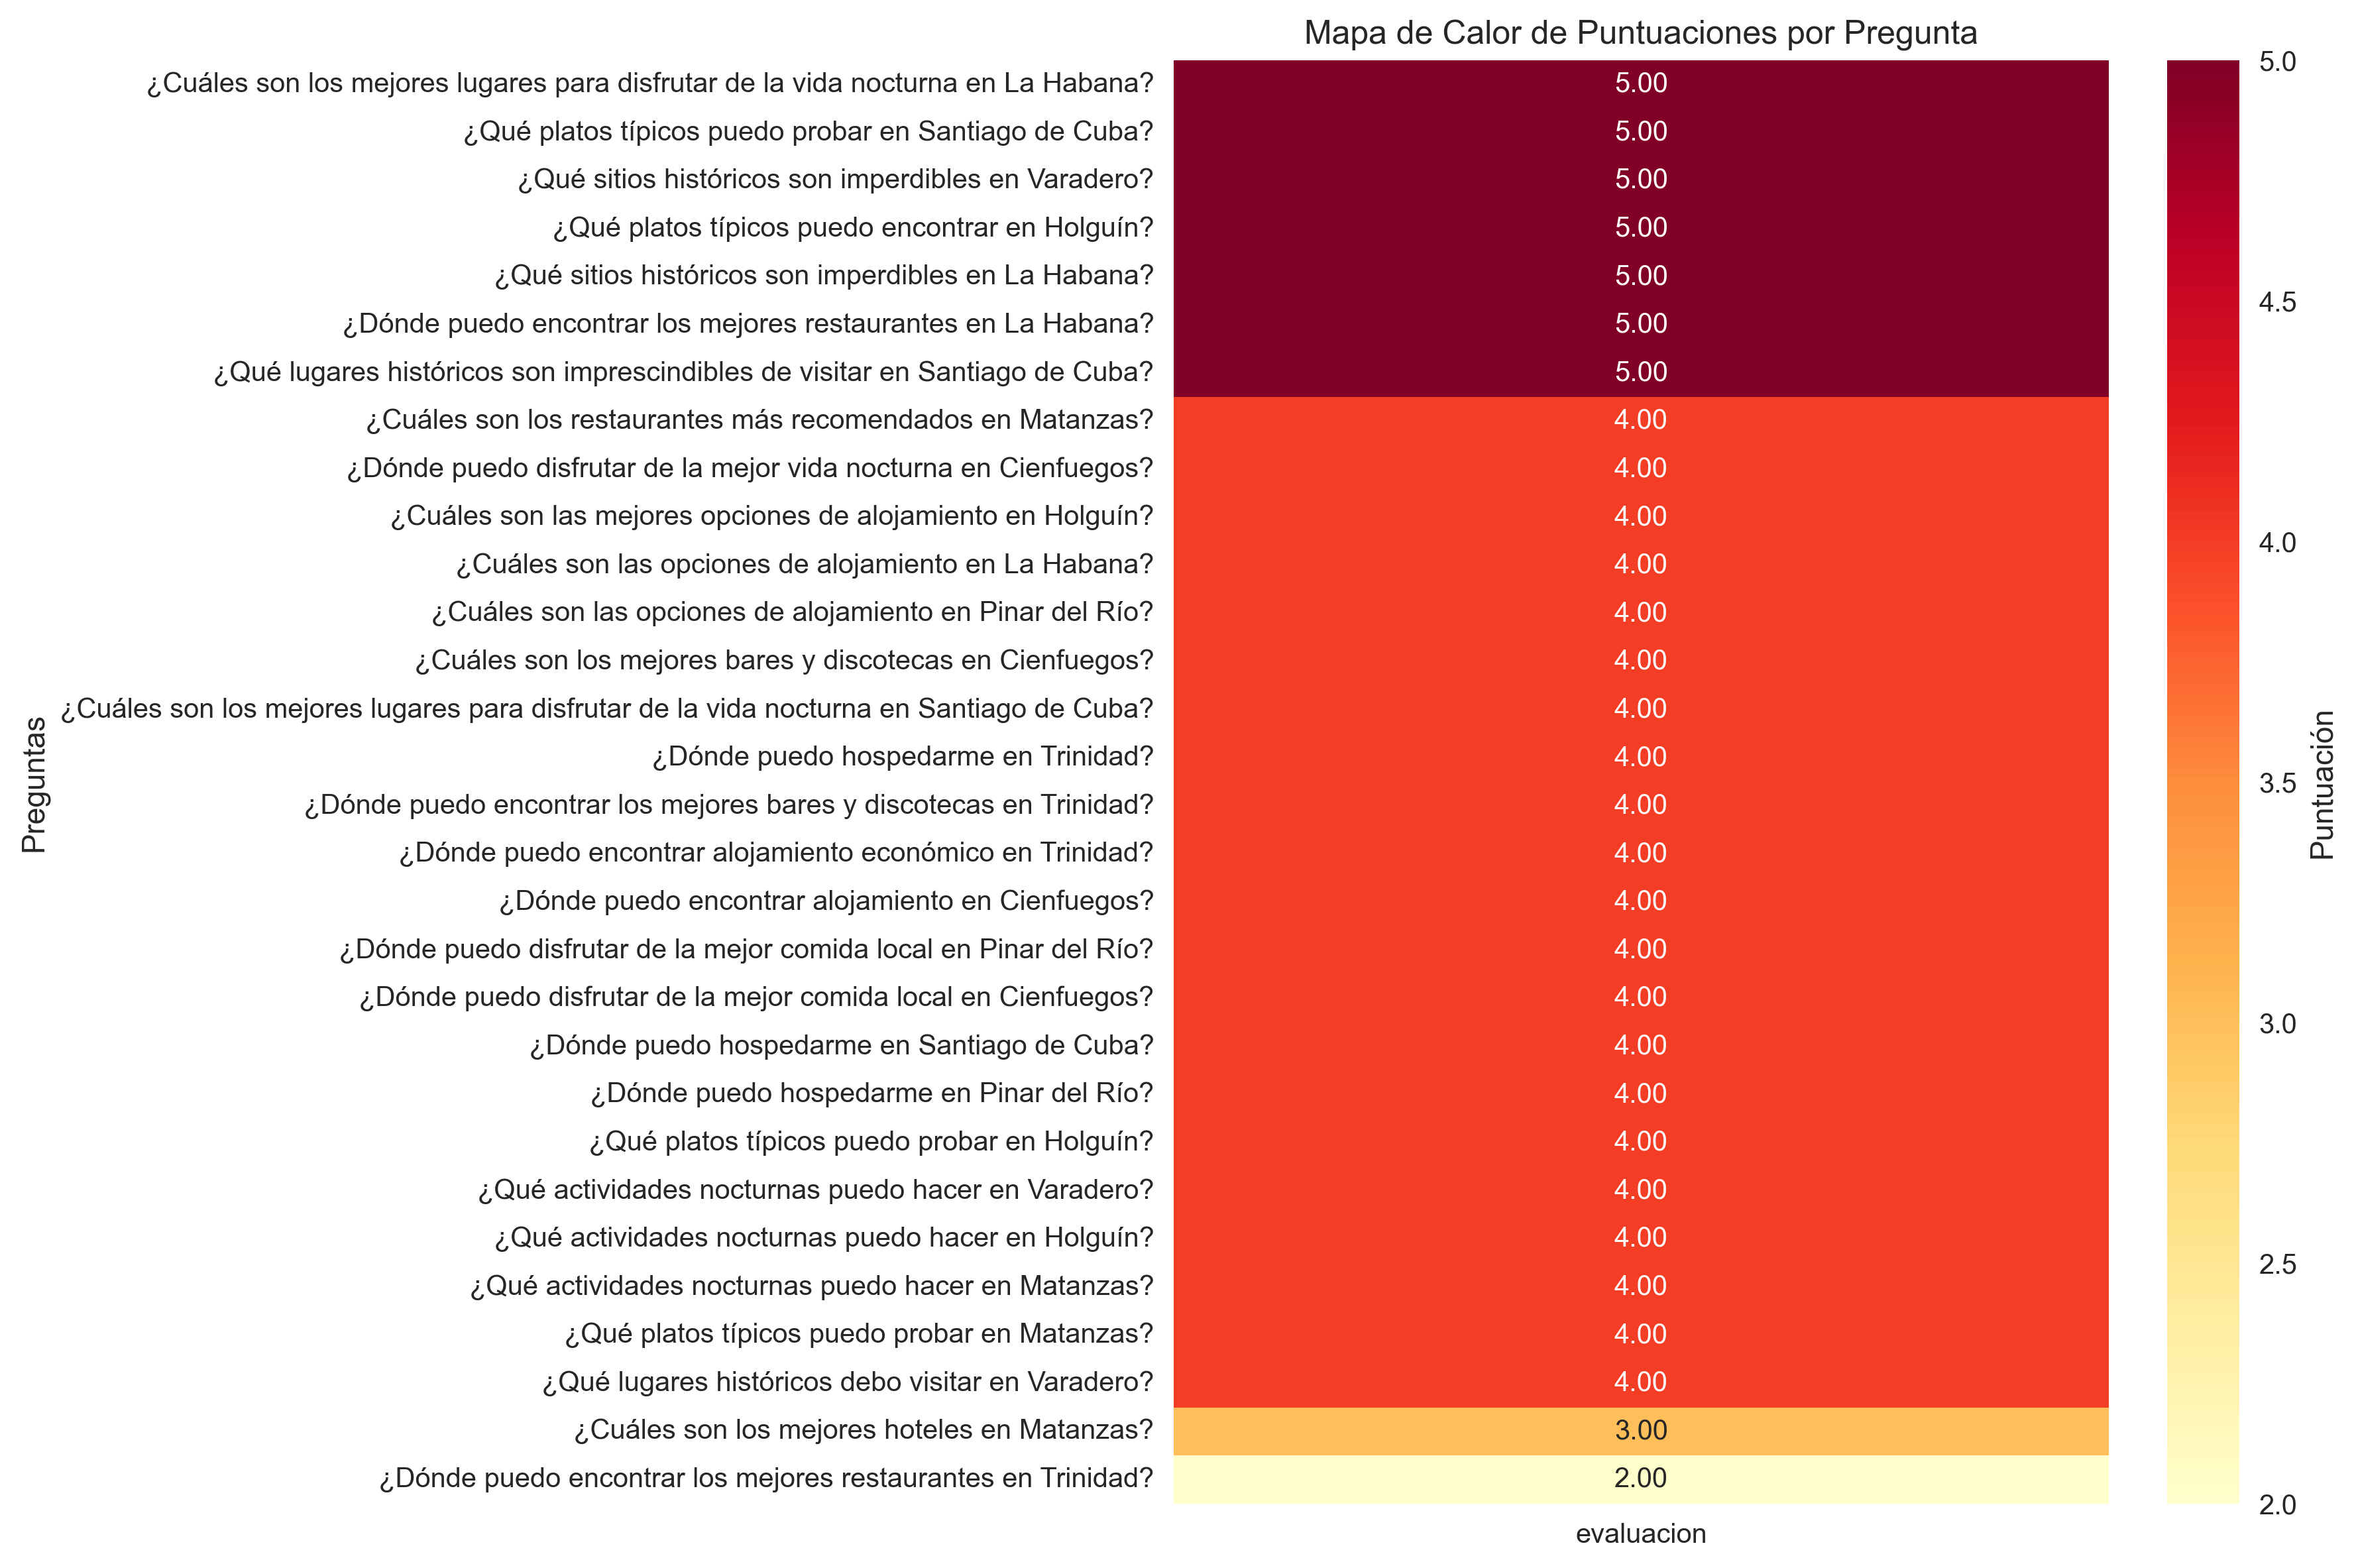
\includegraphics[width=1\textwidth]{../src/experiments/specialized_agents/quality_heatmap_20250617-171856.png}
\caption{Evaluaciones obtenidas para la respuesta a cada pregunta en la muestra inicial (tamaño 30)}
\label{fig:eval_2}
\end{figure}

% --- Apéndice B ---
\newpage
\section{Algoritmos}

\begin{algorithm}
\caption{Generación de Vecino}
\label{alg:nb_gen}
\begin{algorithmic}[1]
\Procedure{GenerateNeighbor}{$sol$}
\State $day \gets \text{random}(0, \text{len}(sol)-1)$
\State $activity \gets \text{random.choice}(\text{actividades})$
\If{$activity \in \{\text{desayuno}, \text{almuerzo}, \text{cena}\}$}
    \State $new\_place \gets \text{random.choice}(\text{lugares\_gastronomicos})$
\ElsIf{$activity = \text{noche}$}
    \State $new\_place \gets \text{random.choice}(\text{lugares\_nocturnos})$
\Else
    \State $new\_place \gets \text{random.choice}(\text{alojamientos})$
\EndIf
\State $sol[day][activity] \gets new\_place$
\State \textbf{return} $sol$
\EndProcedure
\end{algorithmic}
\end{algorithm}

\begin{algorithm}
\caption{Validación de Solución}
\label{alg:sol_valid}
\begin{algorithmic}[1]
\Procedure{IsValidSolution}{$sol$}
\For{$day$ in $sol$}
    \State $total\_cost \gets 0$
    \For{$activity$ in $day$}
        \State $total\_cost \gets total\_cost + day[activity].cost$
    \EndFor
    \If{$total\_cost > budget\_per\_day$}
        \State \textbf{return} False
    \EndIf
\EndFor
\State \textbf{return} True
\EndProcedure
\end{algorithmic}
\end{algorithm}

\begin{algorithm}
\caption{Algoritmo de Recocido Simulado para Planificación de Itinerarios}
\label{alg:recocido_viajes}
\begin{algorithmic}[1]
\Require $days \geq 1$, $places \neq \emptyset$, $budget\_per\_day > 0$, $max\_iter > 0$, $max\_time > 0$
\Ensure Solución óptima de itinerario válido
\Statex
\Function{SimulatedAnnealingCSP}{$days$, $places$, $budget\_per\_day$, $destination$, $max\_iter$, $max\_time$}
\State $start\_time \gets \text{time.now()}$
\State $current\_sol \gets \text{generate\_initial\_solution()}$ \Comment{Solución aleatoria inicial}
\State $best\_sol \gets \text{copy}(current\_sol)$
\State $best\_rating \gets \text{calculate\_total\_rating}(current\_sol)$
\State $T \gets 100.0$ \Comment{Temperatura inicial}
\State $\alpha \gets 0.99$ \Comment{Factor de enfriamiento}
\State $T_{min} \gets 0.1$ \Comment{Temperatura final}

\While{$T > T_{min}$ \textbf{and} $\text{time.now()} - start\_time < max\_time$}
    \For{$i = 1$ \textbf{to} $max\_iter$}
        \If{$\text{time.now()} - start\_time \geq max\_time$}
            \State \Return $best\_sol$ \Comment{Tiempo límite alcanzado}
        \EndIf
        
        \State $neighbor\_sol \gets \text{generate\_neighbor}(current\_sol)$
        \If{$\text{not is\_valid\_solution}(neighbor\_sol)$}
            \State \textbf{continue} \Comment{Descarta soluciones inválidas}
        \EndIf
        
        \State $\Delta \gets \text{calculate\_total\_rating}(neighbor\_sol) - \text{calculate\_total\_rating}(current\_sol)$
        
        \If{$\Delta > 0$ \textbf{or} $\text{random()} < \exp(\Delta / T)$}
            \State $current\_sol \gets neighbor\_sol$
            \If{$\text{calculate\_total\_rating}(current\_sol) > best\_rating$}
                \State $best\_sol \gets \text{copy}(current\_sol)$
                \State $best\_rating \gets \text{calculate\_total\_rating}(current\_sol)$
            \EndIf
        \EndIf
    \EndFor
    \State $T \gets \alpha \times T$ \Comment{Enfriamiento}
\EndWhile

\State \Return $best\_sol$
\EndFunction
\end{algorithmic}
\end{algorithm}

\end{document}